\documentclass[french]{book}
\usepackage[utf8]{inputenc}
\usepackage[explicit, clearempty]{titlesec}
\titleformat{\chapter}[display]{\bfseries\filright}{\huge\chaptername~\thechapter}{20pt}{\Huge#1}
\titleformat{name=\chapter, numberless}[display]{\bfseries\filright}{}{0pt}{\Huge#1}[\addcontentsline{toc}{chapter}{#1}]

\usepackage[T1]{fontenc}
\usepackage{graphicx}
\usepackage[french]{babel}
\usepackage{tabu}


\title{Cahier des charges}

\author{Brahim BAHAIDA}

\date{Mercredi 16 janvier 2019}


\begin{document}

\begin{titlepage}
\maketitle
\thispagestyle{empty}
\end{titlepage}

\tableofcontents


%%%%%%%%%%%%%%%%%%%%%%%%%%%%%%%%%%%%%%%%%%%%%%%%%%%%%%%%%%%%%%%%%%%%%%%%%%%%%%%%%%%%%%%%%%%%%%%%%%%%%%%%%%%%%%%%%%%%%%%%%%%%%%%%%%%%%%
\chapter*{Introduction}

Ce document a pour but d'expliquer le contexte et les exigences du projet et pour cela nous commencerons par une vision globale du projet et ensuite nous présenterons les spécifications du projet.
\section*{liste de diffusion}
\begin{tabu} to 0.8\textwidth { | X[c] | X[c] | }
 \hline
 \textbf{Prénom et Nom} & \textbf{Rôle} \\
 \hline
 Ghassen HAMROUNI  & Encadrant profissionnel \\
\hline
Rim KAABI  & Encadrant académique \\
\hline
Brahim BAHAIDA  & Réalisateur du projet \\
\hline

\end{tabu}

\section*{suivi des versions}

\begin{tabu} to 0.8\textwidth { | X[c] | X[c] | }
 \hline
 \textbf{Version} & \textbf{Dernière modification} \\
 \hline
 1.0  & 16/01/2019 \\
\hline
\end{tabu}

\section*{glossaire}

\begin{tabu} to 0.8\textwidth { | X[c] | X[c] | }
 \hline
 \textbf{Acronyme} & \textbf{Signification} \\
 \hline
 DQM  & Data Quality Management \\
\hline
DFD  & Data Flow Diagrams \\
\hline
\end{tabu}
\\
\chapter{Vision globale du projet}
Ce chapitre vise à présenter le contexte, le planning et les contraintes du projet.
\section{Description du projet}

L'objectif de ce projet est de concevoir et de développer une plateforme de gestion et d'amélioration de la qualité des données clients pour les institutions financières afin d'améliorer leur conformité réglementaire.
\\
\\
Nous utiliserons le diagramme de contexte de la technique DFD (Data Flow Diagrams) pour illustrer les fonctionnalités de la plate-forme. 
\\
\\
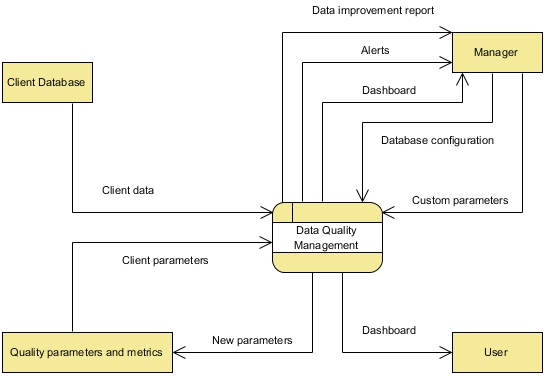
\includegraphics[width=\textwidth]{img/Context_DFD.jpg}\\
\\


\section{Planning}

\section{Contraintes}
bla bla bla

\subsection{Accessibilité}
\subsection{SEO}
\subsection{Responsive design}
\subsection{Applications et librairies tierces}
\subsection{Sécurité}




\section{Public de la plate-forme}
bla bla
    \begin{itemize}
        \item \textbf{Manager} bla bla bla
        \item \textbf{User} bla bla bla
    \end{itemize}
    
\chapter{Les spécifications du projet}

\section{Specifications fonctionnelles} 

\section{Specifications techniques} 

\end{document}